\section{Literature Review}
% \textit{What is the problem to be solved, and it's significance?
% \begin{itemize}
%     \item Brief background to project
%     \item Summary of literature relevant to project
%     \item Identification of "gaps" in the literature
% \end{itemize}}

% The literature review is not just about presenting descriptions of the important papers you have found, but telling a meaningful story and, where appropriate, some critical discussion of previous findings (i.e. was another study useful but flawed?). Remember that you may read hundreds of papers/books/web pages etc., but often only about 20 or 30 are really important, and these are the ones you will mention in your literature review, which this report will be a concise version of. This section needs to flow logically, and this does not always imply that the material is chronological. By the end, the reader should have a clear appreciation of what the major work in the field was, why it is relevant to the current project, and where the unknowns and questions lie (\textbf{research gaps}) – these are the issues that you are going to address with your thesis research.

% For the purposes of this report, this section will be \textbf{12-15 pages long}. Remember to reference properly any material that you obtain from literature or other sources. If you are unsure how to discuss literature properly, find a really good review paper on your topic, or if there isn’t one, a similar topic, and you will have a good example to refer to.

\subsection{Principles of Photovoltaic Modules}
% Photovoltaic Module Definition
Photovoltaic modules, commonly known as solar panels, are devices that convert sunlight into electrical energy. \cite{EnelGreenPowerPhotovoltaicModule}\cite{U.S.DEPARTMENTofENERGY2024SolarBasics}\vspace{0.5em}

% Photoelectric Effect
\noindent Sunlight is made up of massless particles called photons, which possess a certain amount of energy. When these photons strike the surface, they knock electrons off of it, known as photoelectrons. This is known as the photoelectric effect, shown in Figure \ref{fig:photoelectric_effect_diagram}.\vspace{0.5em}

\begin{figure}[ht]
    \centering
    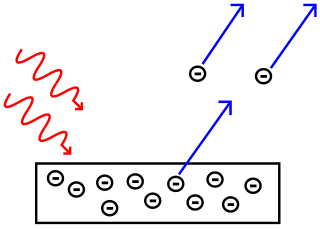
\includegraphics[width=0.4\textwidth]{Figures/photoelectric_effect_diagram.png}
    \caption{Photoelectric Effect Diagram. \cite{KhanAcademyPhotoelectricEffect}}
    \label{fig:photoelectric_effect_diagram}
\end{figure}
\FloatBarrier

\noindent The photoelectric effect will occur only if the frequency of the radiation is greater than the threshold frequency of the metal. The threshold frequency is the minimum frequency of light that causes electrons to be emitted from a material. The proportional relationship that exists between the threshold frequency and the work function is shown in Equation \ref{eq:work_function}.
\begin{equation}
    E = hf_0
    \label{eq:work_function}
\end{equation}

\noindent The work function refers to the minimum amount of energy needed to remove an electron from a metal surface. If photons with enough energy hit the surface, they can transfer their energy to the electrons allowing them to escape. If the energy of the incident photons is less than the work function, no electrons will be emitted, regardless of the intensity of the light. \cite{ScienceABC2023PhotoelectricBeginners}\vspace{0.5em}

% An Explanation of How Photovoltaic Modules Work
\noindent A photovoltaic module is made up of multiple photovoltaic cells, commonly known as solar cells. Each photovoltaic cell is made of semiconductor material, which is placed between the conductive layers. The most common semiconductor material used to make photovoltaic cells is silicon, accounting for 95 percent of photovoltaic modules sold worldwide. \cite{U.S.DEPARTMENTofENERGYSolarBasics} These photovoltaic cells use the photovoltaic effect to convert solar energy into electrical energy.\vspace{0.5em}

\noindent As shown in Figure \ref{fig:photovoltaic_cell_diagram}, a silicon photovoltaic cell is composed of two different layers of silicon: an n-type silicon layer, which has additional electrons, and a p-type silicon layer, which has extra spaces for the electrons, called holes.\par

\noindent ADD IN THE STUFF ABOUT DOPING (CAN BE FOUND IN BARRY'S SECOND PARAGRAPH IN 2.1.)

\begin{figure}[ht]
    \centering
    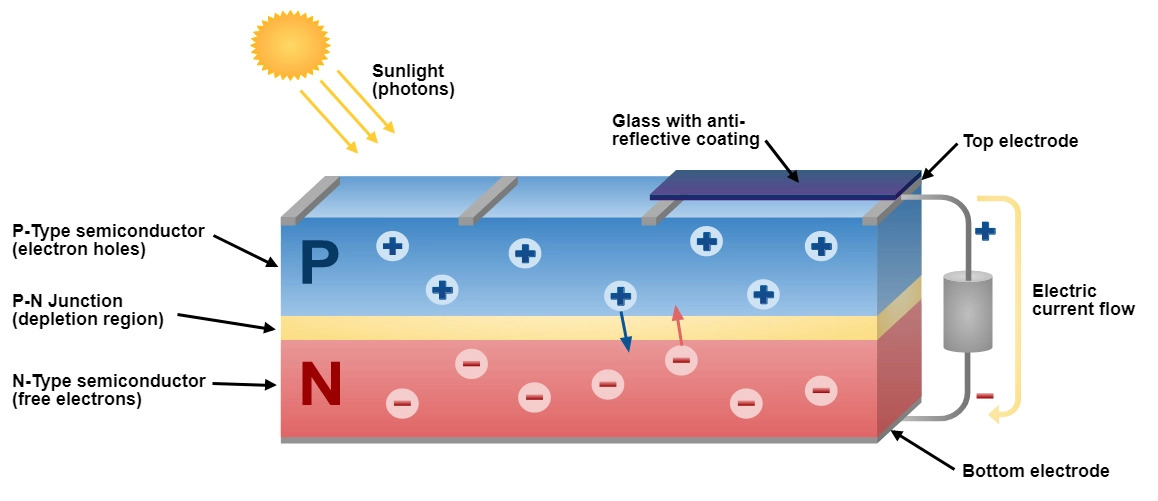
\includegraphics[width=1\textwidth]{Figures/photovoltaic_cell_diagram.jpg}
    \caption{Photovoltaic Cell Structure Diagram. \cite{Gupta2020SolarVehicle}}
    \label{fig:photovoltaic_cell_diagram}
\end{figure}
\FloatBarrier

\noindent When a proton strikes the silicon photovoltaic cell with the required energy, an electron is knocked out of its bond. Because of the electric field at the p-n junction, the negatively charged electron moves toward the n-side, while the resulting positively charged hole is attracted to the p-side. The free electrons are collected by thin metal fingers positioned at the top of the photovoltaic cell, before travelling through an external circuit. After electrical work is performed, the electrons are returned to the conductive aluminium sheet positioned at the back of the photovoltaic cell. Since electrons follow a continuous cycle and are the only moving components, there is no wear and tear, allowing photovoltaic cells to last for decades. \cite{TED-Ed2016HowKomp} However, they still have limitations.\vspace{0.5em}

\pagebreak
\subsection{Performance Limitations of Photovoltaic Modules}
A major limitation of photovoltaic modules is their declining electrical efficiency, particularly at high temperatures. A review led by Swapnil Dubey of Nanyang Technological University found that standard photovoltaic modules typically convert 6-20\% of incoming solar radiation into electrical energy. The remaining 80-94\% is mostly converted into heat, increasing the module’s temperature and further lowering its efficiency. \cite{Dubey2013TemperatureReview}\vspace{0.5em}

% An active cooling system for photovoltaic modules - H.G. Teo
\noindent A 2010 study led by H.G. Teo from the National University of Singapore refined Dubey et al.'s electrical efficiency range to 8-14\%. In the study, Teo et al. focused on comparing the electrical efficiency of photovoltaic modules under cooling and non-cooling conditions.\par\vspace{0.5em}

\noindent Teo et al. observed that the electrical efficiency of the photovoltaic module decreased as the temperature of the module increased, as shown in Figure \ref{fig:electrical_efficiency_vs_temperature_pv_module}. Teo et al. also found that without active cooling, the module temperature was significantly higher than when active cooling was applied under the same meteorological conditions. Thus, active cooling improved the module’s electrical efficiency from 8–9\% to 12–14\%. \cite{Teo2012AnModules}

\begin{figure}[ht]
    \centering
    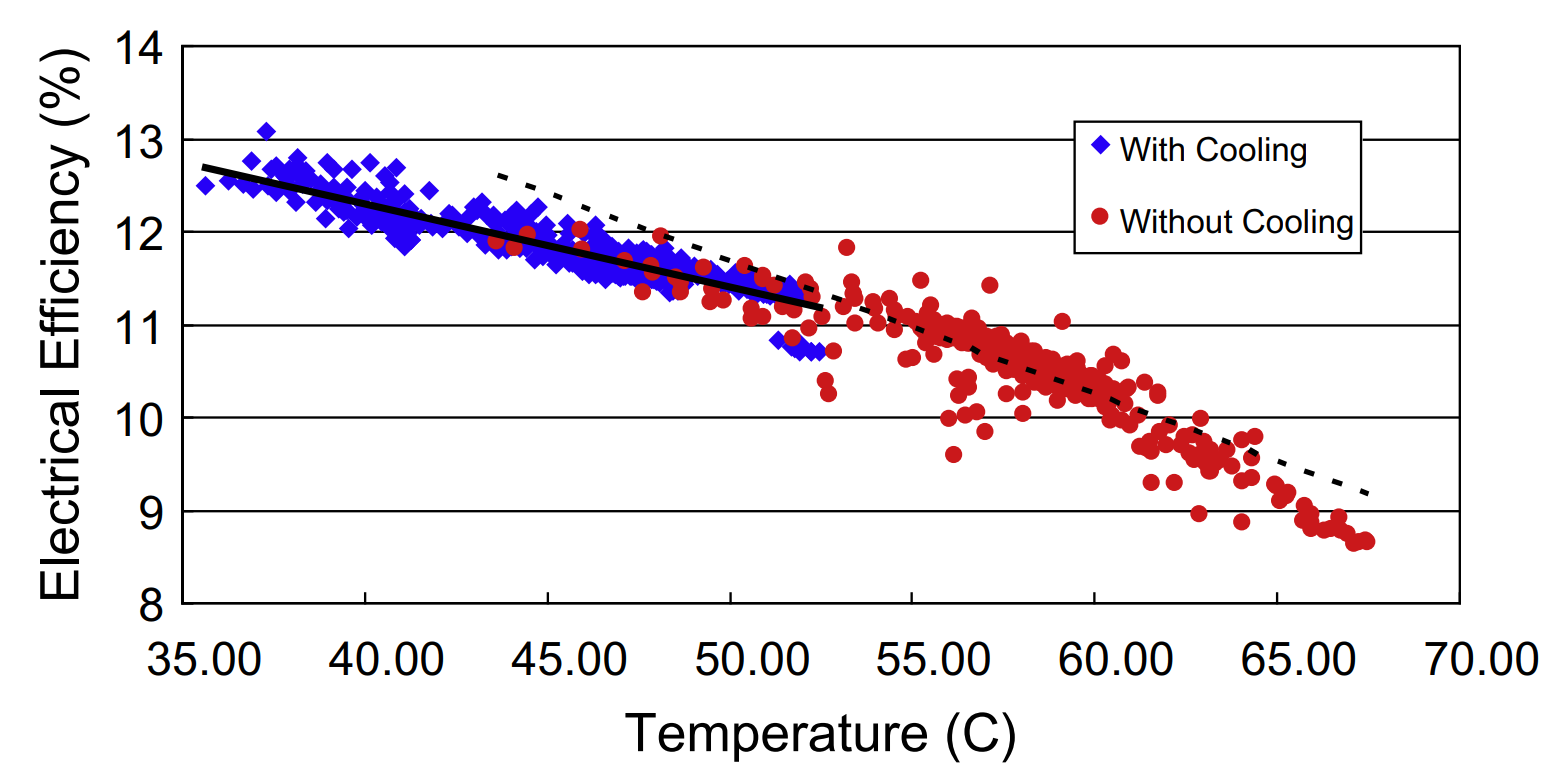
\includegraphics[width=0.7\textwidth]{Figures/electrical_efficiency_vs_temperature_pv_module.png}
    \caption{Electrical efficiency as a function of PV temperature. \cite{Teo2012AnModules}}
    \label{fig:electrical_efficiency_vs_temperature_pv_module}
\end{figure}
\FloatBarrier

\noindent The inverse linear relationship between the temperature and the electrical efficiency of a photovoltaic module is attributed to the band gap reduction, which occurs as the module's temperature increases.\vspace{0.5em}

% An explanation as to how increased module temperature leads to band gap reduction
\noindent In 1931, A.H. Wilson's paper, \textit{The Theory of Electronic Semi-Conductors}, introduced the idea that semiconductors have a small but finite band gap that affects their electrical conductivity. \cite{Il1931TheSemi-Conductors} The band gap represents the amount of energy that an electron must possess to jump from the valence band, where valence electrons are confined, to the conduction band. When valence electrons receive enough energy from an external source, they are able to undergo this band transition, which allows the material to conduct electricity. \cite{CircuitBread2018BandElectronics} As the temperature of the photovoltaic module increases, the valence electrons in the semiconductor material are excited. Thus, the energy required for an electron to transition from the valence band to the conduction band decreases, as indicated by a reduction in the band gap. \cite{Renewable_Tek2025HOTExplained} \par\vspace{0.5em}

% Electrical efficiency of a photovoltaic module
\noindent To understand the proportional relationship between the band gap and the electrical efficiency, an inspection of the formula used to calculate the electrical efficiency of a photovoltaic cell, shown in Equation \ref{eq:pv_cell_efficiency_function}, is required. \cite{HonsbergSolarEfficiency}

\begin{equation}
    \eta = \frac{V_\text{OC}I_\text{SC}FF}{P_\text{in}}
    \label{eq:pv_cell_efficiency_function}
\end{equation}

\noindent The open circuit voltage, short circuit current and fill factor are all affected by the band gap. Therefore, an investigation into the effect of a reduced band gap on these aforementioned variables is necessary to evaluate the impact that the band gap has on the electrical efficiency of the photovoltaic module.\par\vspace{0.5em}

% Open circuit voltage
\noindent A 1994 study led by P. Baruch from the University of Paris derived a formula for determining the minimum value of the diode saturation current, as shown in Equation \ref{eq:minimum_diode_saturation_current}.

\begin{equation}
    J_0 = \frac{q}{k} \frac{15\sigma}{\pi^4} T^3 \int_{u}^{\infty} \frac{x^2}{e^x - 1}\,dx
    \label{eq:minimum_diode_saturation_current}
\end{equation}

\noindent where $u = \frac{E_G}{kT}$. \cite{Baruch1995OnConversion} A casual inspection of Equation \ref{eq:minimum_diode_saturation_current} shows a relationship between the band gap energy and the diode saturation current. However, it is not immediately obvious what the nature of the relationship is due to the complexity of the integral function.\vspace{0.5em}

\noindent Just over a decade later, Michael Y. Levy and Christiana Honsberg from the University of Delaware proposed a method to evaluate the integral in Baruch's formula. \cite{Levy2006RapidApplications} Then, in 2017, Honsberg worked with Stuart Bowden to graph the relationship between the diode saturation current and the band gap based on this method, as shown in Figure \ref{fig:diode_saturation_current_bandgap_graph}.\par

\begin{figure}[ht]
    \centering
    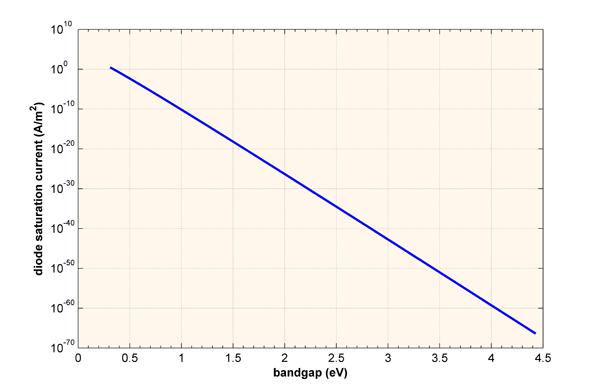
\includegraphics[width=0.7\textwidth]{Figures/diode_saturation_current_bandgap_graph.png}
    \caption{Diode saturation current as a function of band gap. The values are determined from detailed balance and place a limit on the open circuit voltage of a solar cell. \cite{HonsbergOpen-CircuitVoltage}}
    \label{fig:diode_saturation_current_bandgap_graph}
\end{figure}
\FloatBarrier

\noindent Honsberg and Bowden used the diode saturation current values, $J_0$, from Figure \ref{fig:diode_saturation_current_bandgap_graph}, denoted as $I_0$ in Equation \ref{eq:open_circuit_voltage_function}, to calculate the open-circuit voltage as a function of the band gap. The linearly proportional relationship between the band gap and the open-circuit voltage is shown in Figure \ref{fig:open-circuit_voltage_bandgap_graph}.

\begin{equation}
    V_{OC} = \frac{n k T}{q} \times \ln\left(\frac{I_L}{I_0} + 1\right)
    \label{eq:open_circuit_voltage_function}
\end{equation}

\begin{figure}[ht]
    \centering
    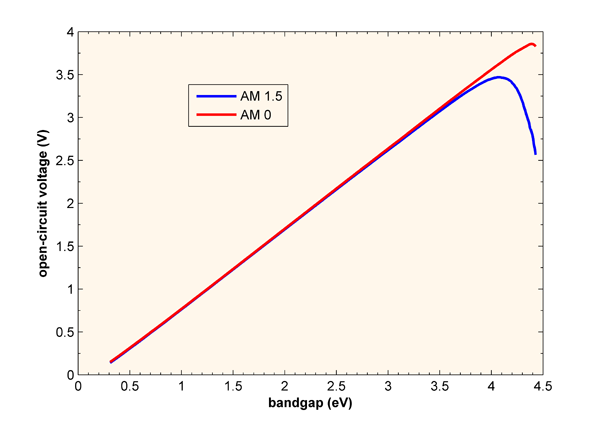
\includegraphics[width=0.7\textwidth]{Figures/open-circuit_voltage_bandgap_graph.png}
    \caption{$V_\text{OC}$ as a function of band gap for a cell with AM 0 and AM 1.5. The $V_\text{OC}$ increases with bang gap as the recombination current falls. There is drop off in $V_\text{OC}$ at very high band gaps due to the very low $I_\text{SC}$. \cite{HonsbergOpen-CircuitVoltage}}
    \label{fig:open-circuit_voltage_bandgap_graph}
\end{figure}
\FloatBarrier

\noindent Thus, the reduced band gap due to the increased temperature of the photovoltaic module leads to a decrease in the open-circuit voltage. \cite{HonsbergOpen-CircuitVoltage}\vspace{0.5em}

\pagebreak
% Short circuit current
\noindent Honsberg and Bowden also graphed the relationship between the band gap and the short circuit current density, as shown in Figure \ref{fig:short_circuit_current_density_bandgap_graph}.

\begin{figure}[ht]
    \centering
    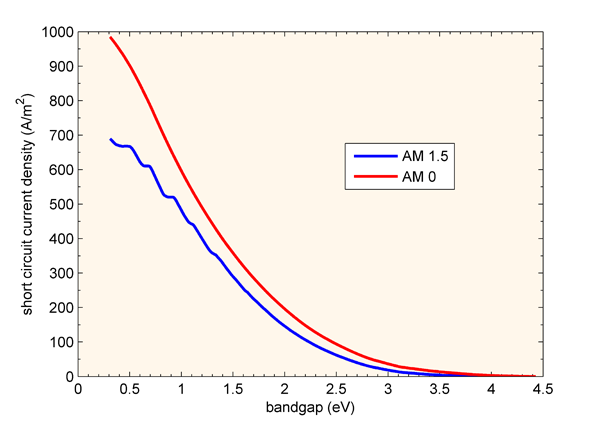
\includegraphics[width=0.7\textwidth]{Figures/short_circuit_current_density_bandgap_graph.png}
    \caption{$J_\text{SC}$ as a function of band gap for a cell with AM 0 and AM 1.5. \cite{HonsbergShort-CircuitCurrent}}
    \label{fig:short_circuit_current_density_bandgap_graph}
\end{figure}
\FloatBarrier

\noindent From Figure \ref{fig:short_circuit_current_density_bandgap_graph}, it is evident that a band gap reduction corresponds to an increase in the short circuit current density. Equation \ref{short_circuit_current_function} shows a linearly proportional relationship between the short circuit current and the short circuit current density.

\begin{equation}
    I_\text{SC} = J_\text{SC}A
    \label{short_circuit_current_function}
\end{equation}

\noindent Therefore, a decrease in the band gap leads to an increase in the short-circuit current. \cite{HonsbergShort-CircuitCurrent}\vspace{0.5em}

% Fill Factor
\noindent In 1981, M.A. Green of the University of New South Wales proposed an empirical expression for the fill factor, as shown in Equation \ref{eq:fill_factor_function}.

\begin{equation}
    FF = \frac{v_\text{OC} - ln(v_\text{OC} + 0.72)}{v_\text{OC} + 1}
    \label{eq:fill_factor_function}
\end{equation}\vspace{0em}

\noindent where $v_\text{OC}$ is defined as a normalised $V_\text{OC}$: $v_\text{OC} = \frac{q}{nkT} V_\text{OC}$. \cite{Green1981SolarExpressions}\vspace{0.5em}

\noindent As established earlier in Figure \ref{fig:open-circuit_voltage_bandgap_graph}, a band gap reduction corresponds to a decrease in the open-circuit voltage. An evaluation of Equation \ref{eq:fill_factor_function} reveals that a decline in the open-circuit voltage and an increase in the temperature of the photovoltaic module causes a decrease in the fill factor. Therefore, it can be concluded that a band gap reduction causes a decrease in the fill factor.\vspace{0.5em}

% Resultant conclusion
\noindent To summarise, the band gap reduction that arises due to the increased temperature of the photovoltaic module causes a decrease in the open-circuit voltage, an increase in the short circuit current and a decrease in the fill factor. While the short circuit current does increase, it is ultimately outweighed by the decrease in the open-circuit voltage and fill factor, leading to a decrease in the module's electrical efficiency.\vspace{0.5em}

% Additional factors
\noindent In addition to temperature, other environmental factors like shade and air pollution limit the electrical efficiency of photovoltaic modules. A 2013 study led by Alberto Dolara from the Polytechnic University of Milan found that shade significantly affects the performance of photovoltaic modules. Dolara et al. observed a 31\% drop in the power generated by a single photovoltaic cell when 50\% of the cell was subjected to shade. \cite{Dolara2013ExperimentalModules} In 2001, E. Asl-Soleimani et al. from the University of Tehran concluded that air pollution also reduced the energy output of photovoltaic modules by up to 60\%. \cite{Asl-Soleimani2001TheTehran} Furthermore, operational factors like poor module maintenance can lead to dust buildup, significantly reducing power generation. A review led by Khaled Hasan in 2021 stated a 60-70\% reduction in power generation due to the deposition of dust in humid conditions. \cite{Hasan2022EffectsReview} \vspace{0.5em} 

% Link the heat transfer paragraphs to the limitations paragraphs
\noindent In 1961, William Shockley and Hans Queisser published their paper, \textit{Detailed Balance Limit of Efficiency of p-n Junction Solar Cells}, in which they established the theoretical maximum efficiency of silicon-based solar cells to be approximately 30\% under standard illumination conditions. \cite{Shockley1961DetailedCells} In the real world however, photovoltaic cells are prevented from reaching this limit due to the environmental and operational factors previously discussed. Thus, due to the important role that photovoltaic modules play in the future of global energy, methods to reduce the impact that these factors have on the performance of photovoltaic modules are constantly being investigated. In particular, to mitigate the reduction in electrical efficiency caused by increased photovoltaic module temperature, heat transfer-based cooling methods are investigated and employed worldwide.\vspace{0.5em}

\pagebreak
\subsection{Heat Transfer in Photovoltaic Modules}
\noindent The fundamental concept of heat transfer is the process by which heat energy moves from one system or body to another as a result of a temperature difference. This transfer of heat can occur via conduction, convection or radiation. Figure \ref{fig:fundamental_concept_of_heat_transfer_diagram} demonstrates the fundamental concept of heat transfer in the context of a photovoltaic module.\par

\begin{figure}[h]
    \centering
    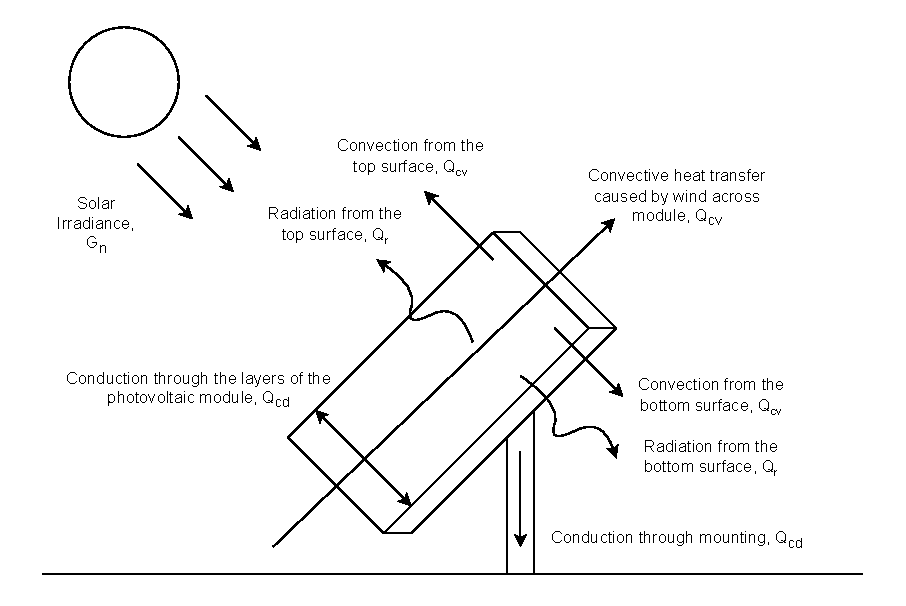
\includegraphics[width=0.75\textwidth]{Figures/fundamental_concept_of_heat_transfer_diagram.pdf}
    \caption{Fundamental concept of heat transfer on a photovoltaic module.}
    \label{fig:fundamental_concept_of_heat_transfer_diagram}
\end{figure}

\noindent In Figure \ref{fig:fundamental_concept_of_heat_transfer_diagram}, conductive heat transfer through the layers of the photovoltaic module and the mounting are observed. Additionally, heat is transferred from the surface of the photovoltaic module to the surrounding air via convection. Finally, the module emits thermal radiation to its surroundings, contributing to radiative heat transfer. In 2020, P. Dwivedi from the Maulana Azad National Institute of Technology, Bhopal, analysed the percentage distribution of heat loss across the different modes of heat transfer, shown in Table \ref{tab:heat_loss_from_pv_module}. \cite{Dwivedi2020AdvancedArt}\par

\begin{table}[ht]
    \centering
    \caption{Heat loss from P.V. module. \cite{Dwivedi2020AdvancedArt}}
    \setlength{\tabcolsep}{50pt} % Adjust column spacing between columns
    \renewcommand{\arraystretch}{1.5} % Increase row height
    \begin{tabular}{@{\hspace{8pt}} l l l @{\hspace{8pt}}}
         \hline
         S.No & Heat loss from module & Percentage \\
         \hline
         1 & Conduction through mounting & 2 \\
         2 & Convection from top surface & 42 \\
         3 & Convection from bottom surface & 24 \\
         4 & Radiation from top surface & 21 \\
         5 & Radiation from bottom surface & 11 \\
         \hline
    \end{tabular}
    \label{tab:heat_loss_from_pv_module}
\end{table}

\noindent Thus, this paper will explore the effectiveness of conduction, convection, and radiation-based cooling methods in lowering the temperature of photovoltaic modules to enhance their overall efficiency.\par

\subsubsection{Conduction} % How does conduction transfer heat in pv modules
\noindent Conduction is the transfer of energy from the more energetic particles of a substance to the adjacent less energetic ones as a result of interactions between the particles. The formula commonly used to calculate the rate of heat conduction is shown in Equation \ref{eq:rate_of_heat_conduction_function}. \cite{Cengel2014HeatApplications}\par

\begin{equation}
    \dot{Q}_\text{cond} = -kA\frac{\Delta T}{\Delta x}
    \label{eq:rate_of_heat_conduction_function}
\end{equation}

\noindent The main conduction-based cooling methods used to reduce photovoltaic module temperatures are finned heat sinks and phase change materials.\vspace{0.5em}

% Finned Heat Sinks
\noindent A heat sink is a component used in thermal management strategies to transfer heat effectively. It's design is optimised to dissipate heat. \cite{Kumar2024QualitativeReview} The use of a heat sink increases the cross-sectional area that the heat is being transferred to, denoted as A in Equation \ref{eq:rate_of_heat_conduction_function}. Through further inspection of Equation \ref{eq:rate_of_heat_conduction_function}, it is observed that the increased cross-sectional area, A, results in an increased rate of conductive heat transfer, $\dot{Q}_\text{cond}$. A study led by S.N. Razali from the National University of Malaysia investigated the effect of multidirectional tapered fin heat sinks (MTFHS) on photovoltaic modules. Razali et al. found that the proposed MTFHS reduced the module's temperature by $12^\circ \text{C}$, indicating enhanced conductive heat transfer, which consequently improved the photovoltaic module's efficiency by 1.53\% \cite{Razali2023PerformanceMTFHS}.\vspace{0.5em}

% Phase Change Materials 
\noindent A phase change material (PCM) is a material that can change its state from solid to liquid and vice versa by releasing and storing thermal energy. \cite{Nicholas2019ActivatedMaterial}\par
\noindent When the surrounding temperature rises above the PCM’s melting point, it liquefies, drawing heat away from the photovoltaic module.\par
\noindent Conversely, when the temperature drops below the melting point, the PCM solidifies, releasing the stored heat back into the environment.\par
\noindent A 2023 study led by B. Hussain of the \par

% Why aren't we focusing on condution (Look at Barry's reason)
\noindent - \par

\subsubsection{Radiation} % How does radiation transfer heat in pv modules
\begin{itemize}
    \item Radiation is the energy that is emitted by matter and is transported as electromagnetic waves (or photons).
\end{itemize}
% \noindent What is radiation?\par
% \noindent How can radiation be used to cool down photovoltaic modules?\par
% \noindent Why are they not the optimal source of heat transfer for cooling down photovoltaic module?\par

\subsubsection{Convection} % How does convection transfer heat in pv modules
\noindent P. Dwivedi et al. observed that convective heat transfer was the primary mode of heat transfer in photovoltaic modules, accounting for 66\% of total heat loss.
\begin{itemize}
    \item Convection is the energy transfer between a solid surface and an adjacent liquid/gas in motion (combines effects of conduction and fluid motion).
\end{itemize}

\paragraph{Natural Convection and the Relevant Cooling Methods (Passive Cooling)} % What role does natural convection play in the convective heat transfer in pv modules
\paragraph{Forced Convection and the Relevant Cooling Methods (Active Cooling)} % What role does natural convection play in the convective heat transfer in pv modules
\subsubsection{Vortex Generators: Vortex Induced Heat Induction} % How are vortices used to induce heat induction

\pagebreak
\subsection{Experimental Techniques}
\subsubsection{Infrared Thermography}
\subsubsection{Thermocouple Sensors}
\subsubsection{Particle Image Velocimetry}

\pagebreak
\subsection{Literature Gap}

\pagebreak

% \subsubsection{Vortex Induced Heat Transfer}
% \begin{itemize}
%     \item What is a vortex?
%     \item How does a vortex/system of vortexes induce heat transfer?
%     \item Are there any drawbacks of vortex-induced heat transfer? If so, what are they?
% \end{itemize}

% \subsubsection{Conduction}
% \begin{itemize}
%     \item What is conduction?
%     \item How can conduction be used to enhance heat transfer?
%     \item What are some examples of this principle in practice?
%     \item What were the results of this practice?
%     \item Are there any drawbacks of conduction as a method to enhance heat transfer?
% \end{itemize}

% \subsubsection{Radiation}
% \begin{itemize}
%     \item What is radiation?
%     \item How can radiation be used to enhance heat transfer?
%     \item What are some examples of this principle in practice?
%     \item What were the results of this practice?
%     \item Are there any drawbacks of radiation as a method to enhance heat transfer?
% \end{itemize}

% \subsection{Convective Photovoltaic Module Cooling Methods}
% \begin{itemize}
%     \item What is convection?
%     \item What are some cooling methods for convective photovoltaic modules?
% \end{itemize}

% \subsubsection{Cooling through Natural Convection}
% \begin{itemize}
%     \item What is Natural Convection?
%     \item How is natural convection used as a cooling method for photovoltaic modules?
%     \item Are there drawbacks to natural convection as a cooling method for photovoltaic modules?
%     \item How does forced convection compare to natural convection as a cooling method for photovoltaic modules?
% \end{itemize}

% \subsubsection{Cooling through Forced Convection}
% \begin{itemize}
%     \item What is forced convection?
%     \item How is forced convection used as a cooling method for photovoltaic modules?
%     \begin{itemize}
%         \item DC Fan Experiment
%         \item Floating Photovoltaic Module Experiment
%     \end{itemize}
%     \item Are there drawbacks to forced convection as a cooling method for photovoltaic modules?
%     \item Air vs Water Cooling Experiment
%     \item Air Cooled Modified Photovoltaic Module Experiment
%     \item Single Fin vs Multiple Fin Experiment
% \end{itemize}

% \subsubsection{Cooling through Vortex Generators}
% \begin{itemize}
%     \item What is a vortex generator?
%     \item What is the purpose of vortex generators?
%     \item Examples of Vortex Generator Experiments in the Context of Photovoltaic Module Cooling
% \end{itemize}